\documentclass{beamer}

\usepackage{graphicx,hyperref,udesc,url}
\usepackage[T1]{fontenc}
\usepackage{booktabs}
\usepackage[portuguese]{babel}
\usepackage[utf8]{inputenc}
\usepackage{hyphenat}
\usepackage{tabularx}
\usepackage{caption}
\newcommand{\source}[1]{\vspace{-6pt} \caption*{Fonte: {#1}} }
\hyphenation{mate-mática recu-perar}
\usepackage{biblatex}
\bibliography{bibliography.bib}

\AtBeginSection[]{
    \begin{frame}
    \vfill
    \centering
    \begin{beamercolorbox}[sep=8pt,center,shadow=true,rounded=true]{title}
        \usebeamerfont{title}\insertsectionhead\par%
    \end{beamercolorbox}
    \vfill
    \end{frame}
}

\title[Aplicação de Diferentes Métodos...]{Aplicação de Diferentes Métodos de Randomização em Meta-heurísticas}

\author[Luiza E. Stadelhofer, Rafael S. Parpinelli]{
    Luiza Engler Stadelhofer, Rafael Stubs Parpinelli\\\medskip
    {\small \url{luiza.engler@gmail.com}} \\ 
    {\small \url{rafael.parpinelli@udesc.br}}}

    \institute[UDESC]{
        Departamento de Ci\^encia da Computa\c{c}\~ao \\
            Centro de Ci\^encias Tecnol\'ogicas\\
            Universidade do Estado de Santa Catarina}
\date{26 de novembro de 2019}
\begin{document}

\begin{frame}
\titlepage
\end{frame}

\begin{frame}
\frametitle{Sumário}
\tableofcontents
\end{frame}

\section{Recapitulo}

\begin{frame}
\frametitle{Problema}
\begin{itemize}
    \item A randomização está fortemente ligada às propriedades de convergência dos algoritmos;
    \item Temos a disposição diversos métodos de randomização que podem ser utilizados;
    \item Grande parte dos estudos não fazem uma análise de qual a melhor distribuição a se usar.
\end{itemize}
\end{frame}

\begin{frame}
\frametitle{Contribuição}
\begin{itemize}
    \item A contribuição deste trabalho se encontra na análise do impacto que diferentes distribuições probabilísticas possuem sobre algumas meta-heurísticas.
\end{itemize}
\end{frame}

\section{Proposta}

\begin{frame}
\frametitle{Motivação}
\begin{itemize}
    \item De acordo com o mapeamento sistemático realizado, existem diversas formas de se aplicar diferentes métodos de randomização em um algoritmo;
    \item Decidiu-se abordar duas dessas aplicações: em todos os pontos de randomização, e em pontos específicos do algoritmo.
\end{itemize}
\end{frame}

\begin{frame}
\frametitle{Aplicação em Todos os Pontos}
\begin{itemize}
    \item Algoritmos: jDE e SCA;
    \item Métodos de randomização: distribuição Uniforme, Gaussiana e mapa caótico Logístico;
    \item Problemas: funções \textit{benchmark} e Predição de Estrutura de Proteínas (PSP).
\end{itemize}
\end{frame}


\begin{frame}
\frametitle{jDE}
\begin{figure}[tbph]
\centering
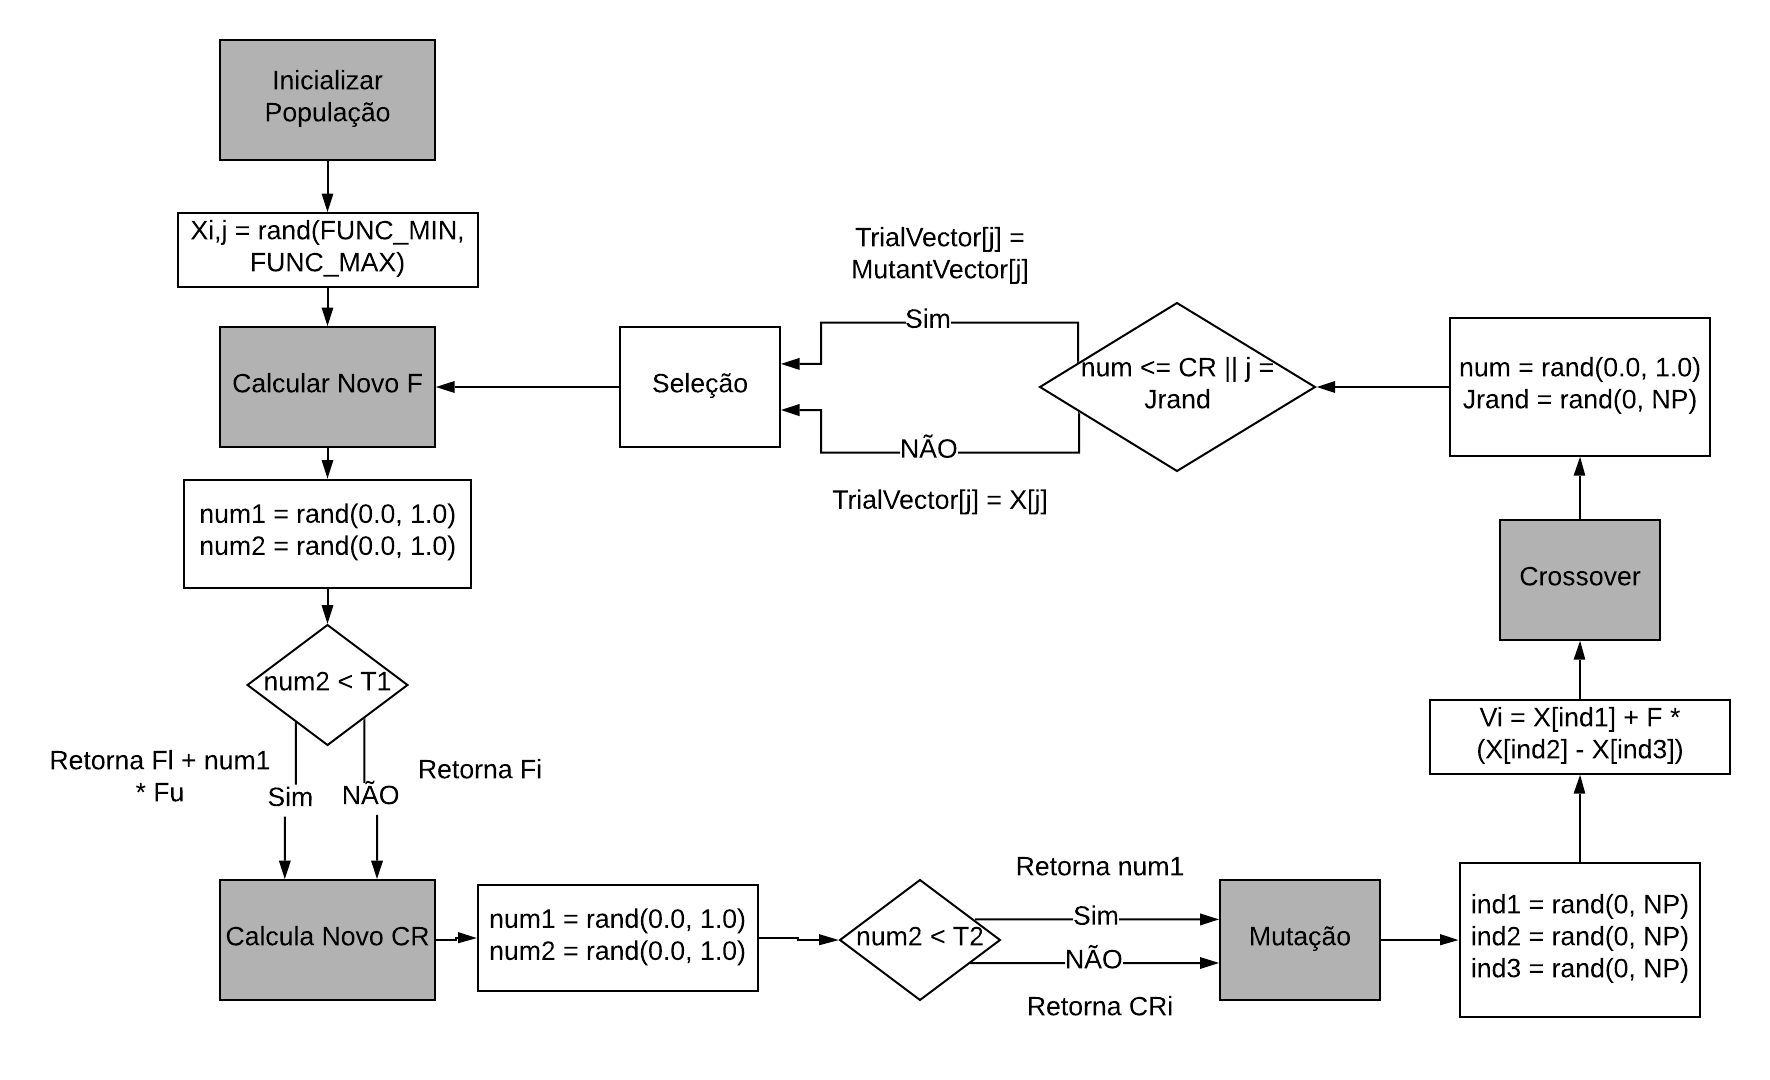
\includegraphics[width=0.9\textwidth]{Diagrama_de_Blocos.png}
\source{Própria autora.}
\label{fig:jDE}
\end{figure}
\end{frame}

\begin{frame}
\frametitle{SCA}
\begin{figure}[tbph]
\centering
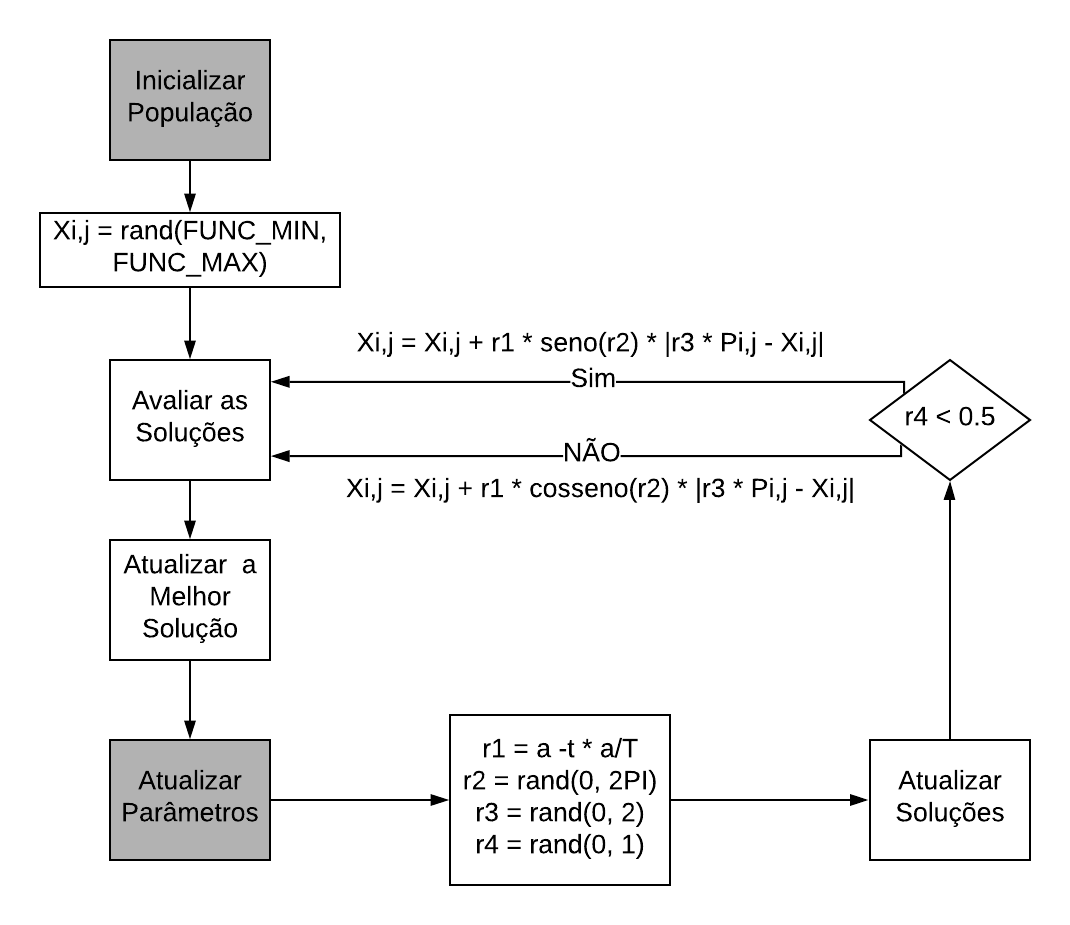
\includegraphics[width=0.6\textwidth]{Diagrama_SCA.png}
\source{Própria autora.}
\label{fig:SCA}
\end{figure}
\end{frame}

\begin{frame}
\frametitle{Aplicação em Pontos Específicos}
\begin{itemize}
    \item O primeiro passo necessário para realizar essa aplicação foi analisar quais parâmetros dos algoritmos são relevantes e possuem um grande impacto no comportamento de intensificação e diversificação dessas meta-heurísticas;
\end{itemize}
\end{frame}

\begin{frame}
\frametitle{Parâmetros SCA}
\begin{table}[!htpb]
    \centering
    \begin{tabularx}{\textwidth}{c|X|c} % <-- Alignments: 1st column left, 2nd middle and 3rd right, with vertical lines in between
    
      \textbf{Parâmetro} & \textbf{Função} &  \textbf{Geração} \\
      \hline
      r1 & Determina a direção do movimento & Auto-adaptado\\
      \hline
      \bf{r2} & Determina o tamanho do movimento & Uniforme [0, 2$\pi$] \\
      \hline
      \bf{r3} & Enfatiza ou não o efeito da melhor solução na definição da distância & Uniforme [0, 2] \\
      \hline
      r4 & Alterna entre as fórmulas de update com seno e cosseno & Uniforme [0, 1] \\
    \end{tabularx}
    \caption{Parâmetros do SCA}
    \label{tab:parametros}
\end{table}
\end{frame}

\begin{frame}
\frametitle{Parâmetro R3}
\begin{itemize}
    \item O parâmetro r3 varia no intervalo de [0, 2], enfatizando (r3 > 1) ou não (r3 < 1) o efeito da melhor solução encontrada até então pelo algoritmo na definição da distância; 
    \item O valor de r3 deve começar baixo e incrementar ao longo das iterações.
\end{itemize}
\end{frame}

\begin{frame}
\frametitle{Parâmetro R3}
\begin{equation}
    \label{eq:desvioR3}
    desvioR3 = 0.0 + iteracaoAtual * \frac{2.0}{maxIteracao}
\end{equation}
\end{frame}

\begin{frame}
\frametitle{Parâmetro R2}
\begin{itemize}
    \item Os termos $r1 * sin(r2)$ e $r1 * cos(r2)$ são os responsáveis por guiar juntamente a habilidade de intensificação e diversificação do algoritmo; 
    \item Valores maiores que 1 ou menores que -1, realizam uma diversificação; enquanto valores no intervalo [-1, 1], realizam um intensificação.
\end{itemize}
\end{frame}

\begin{frame}
\frametitle{Parâmetro R2}
\begin{equation}
\label{eq:mapeamento}
  \begin{gathered}
    2.0 \rightarrow [-2.0, 2.0]\\
    1.9 \rightarrow [-1.9, 1.9]\\
    ...\\
    1.0 \rightarrow [-1.0, 1.0]\\
    ...\\
    0.1 \rightarrow [-0.1, 0.1]\\
    0.0 \rightarrow [0.0, 0.0]\\
 \end{gathered}
\end{equation}
\end{frame}

% \begin{frame}
% \frametitle{Parâmetro R2}
% \begin{itemize}
%     \item Quer-se fazer uma adaptação tal que o valor resultante dos termos $sin(r2)$ e $cos(r2)$ decresça de 1 até -1, consequentemente fazendo com que o algoritmo realize uma diversificação no começo do processo de otimização e uma intensificação no final.
% \end{itemize}
% \end{frame}

\begin{frame}
\frametitle{Parâmetro R2}
\begin{equation}
    \label{eq:desvioR2Sin}
    desvioR2Seno = \frac{\pi}{2} + iteracaoAtual * \frac{(\frac{3\pi}{2}-\frac{\pi}{2})}{maxIteracao}
\end{equation}

\begin{equation}
    \label{eq:desvioR2Cos}
    desvioR2Cosseno = 0.0 + iteracaoAtual * \frac{\pi}{maxIteracao}
\end{equation}
\end{frame}

\section{Experimentos}

\begin{frame}
\frametitle{Configurações - Benchmarks}
\begin{itemize}
    \item Tamanho da população: 30;
    \item Gerações: 2000;
    \item Dimensões: 20;
    \item Execuções: 10;
\end{itemize}
\end{frame}

\begin{frame}
\frametitle{Resultados - Benchmarks}
\begin{figure}[tbph]
\centering
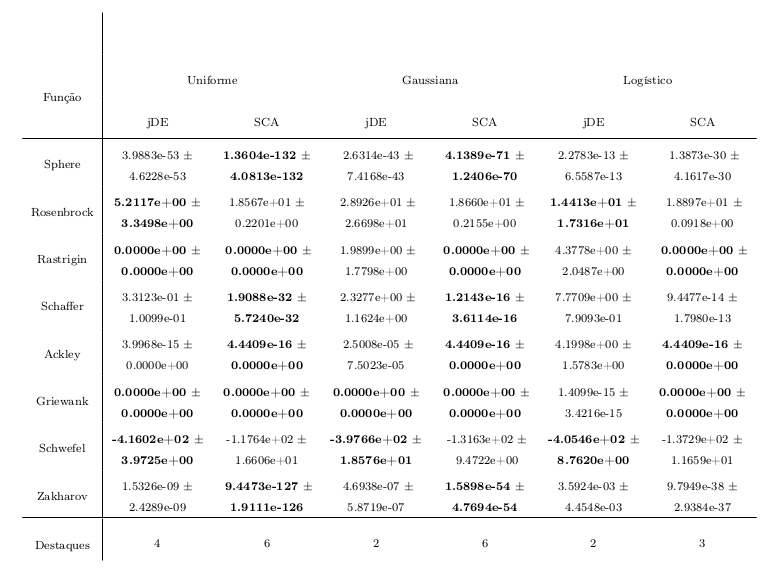
\includegraphics[width=0.8\textwidth]{tabelaBenchmarks1.png}
\source{Própria autora.}
\label{tab:resBench1}
\end{figure}
\end{frame}

% Rastrigin %
\begin{frame}
\frametitle{Resultados - Benchmarks}
\begin{figure}[tbph]
\centering
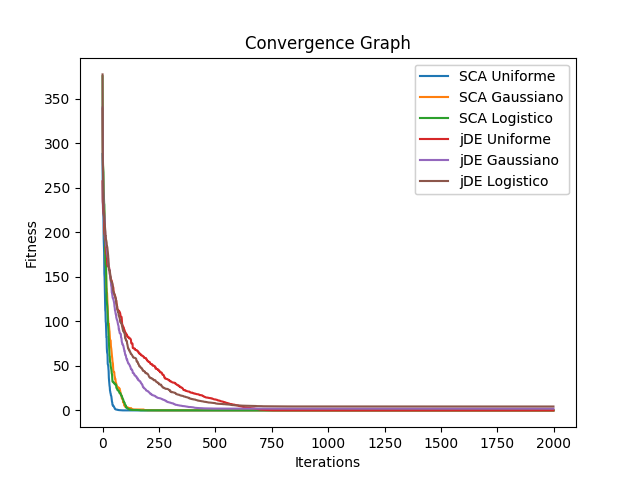
\includegraphics[width=0.49\linewidth]{convRastrigin.png}
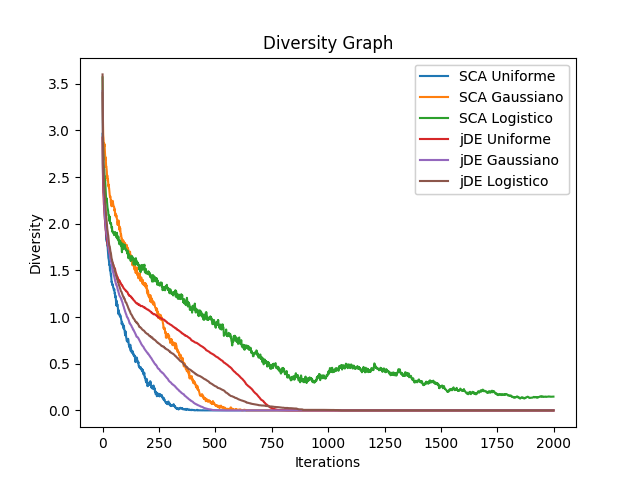
\includegraphics[width=0.49\linewidth]{divRastrigin.png}
\source{Própria autora.}
\label{fig:grafSphere}
\end{figure}
\end{frame}

\begin{frame}
\frametitle{Configurações - PSP}
\begin{itemize}
    \item Tamanho da população: 30;
    \item Gerações: 10000;
    \item Execuções: 30;
\end{itemize}
\end{frame}

\begin{frame}
\frametitle{Resultados - PSP - Todos os Pontos}
\begin{figure}[tbph]
\centering
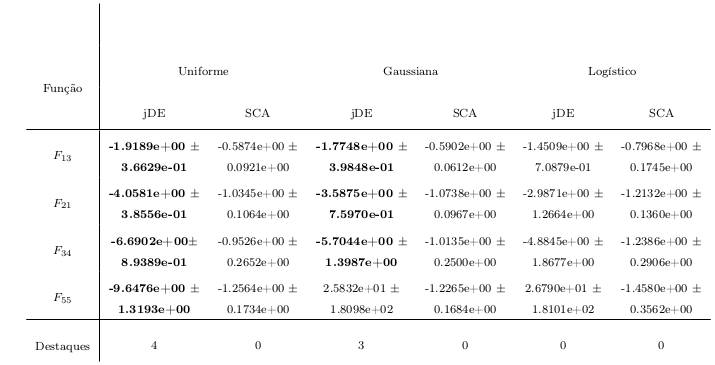
\includegraphics[width=0.9\textwidth]{tabResultadosPSP1.png}
\source{Própria autora.}
\label{tab:resPSP1}
\end{figure}
\end{frame}

% F34 %
\begin{frame}
\frametitle{Resultados - PSP - Todos os Pontos}
\begin{figure}[tbph]
\centering
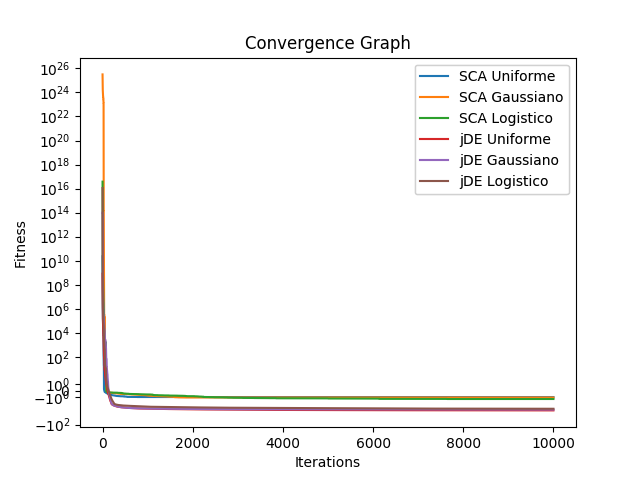
\includegraphics[width=0.49\linewidth]{convF34.png}
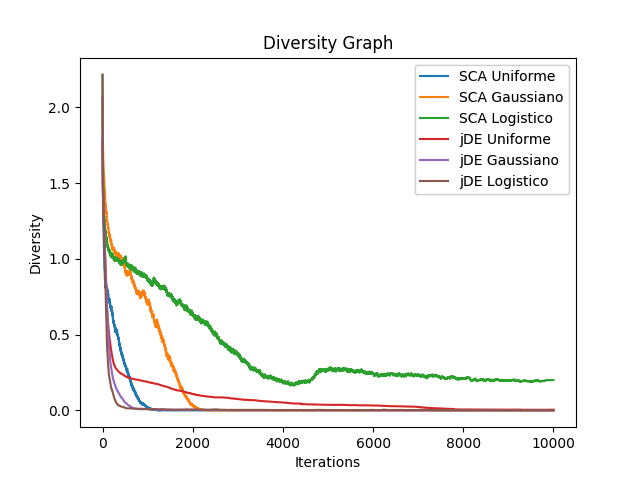
\includegraphics[width=0.49\linewidth]{divF34.png}
\source{Própria autora.}
\label{fig:grafF34}
\end{figure}
\end{frame}

\begin{frame}
\frametitle{Resultados - PSP - Pontos Específicos}
\begin{figure}[tbph]
\centering
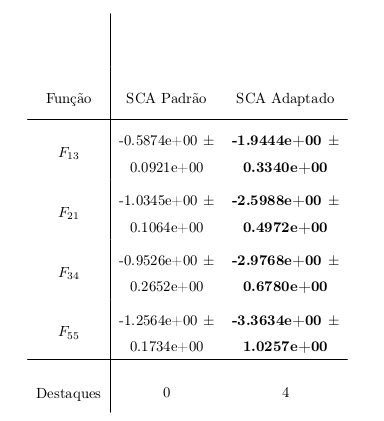
\includegraphics[width=0.5\textwidth]{resultadosPSPAdapt.png}
\source{Própria autora.}
\label{tab:resPSP2}
\end{figure}
\end{frame}

% F34 %
\begin{frame}
\frametitle{Resultados - PSP - Pontos Específicos}
\begin{figure}[tbph]
\centering
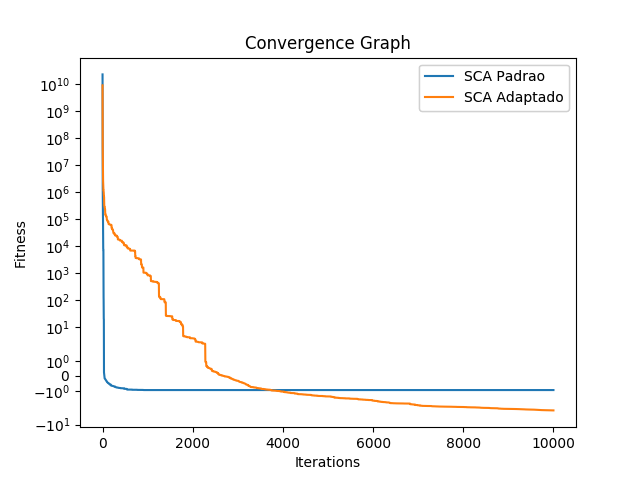
\includegraphics[width=0.49\linewidth]{convF34_F.png}
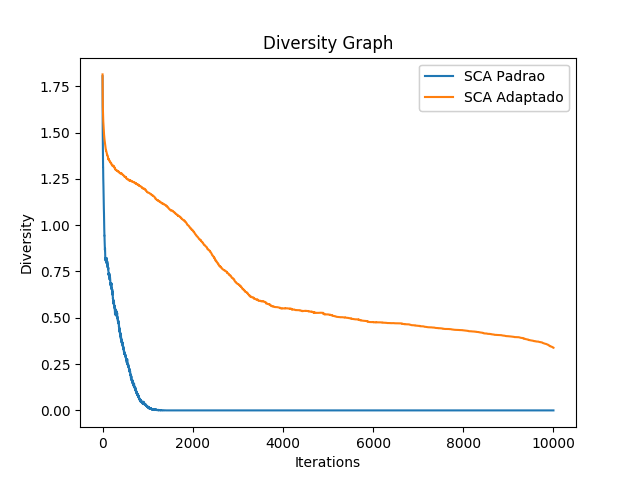
\includegraphics[width=0.49\linewidth]{divF34_F.png}
\source{Própria autora.}
\label{fig:grafF34_F}
\end{figure}
\end{frame}

% \begin{frame}
% \frametitle{Resultados - PSP - Pontos Específicos}
% \begin{figure}[tbph]
% \centering
% 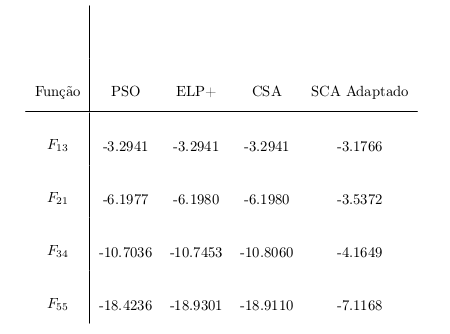
\includegraphics[width=0.6\textwidth]{tabComparacao.png}
% \source{Própria autora.}
% \label{tab:comp}
% \end{figure}
% \end{frame}

\section{Considerações Finais}

\begin{frame}
\frametitle{Considerações Finais}
\begin{itemize}
    \item O método de randomização utilizado para geração de números aleatórios é um parâmetro das meta-heurísticas; 
    \item A decisão, de qual método se utilizar, depende de diversos aspectos, como: o algoritmo que está sendo usado; o problema ao qual o algoritmo está tentando solucionar; e em que partes do algoritmo este método foi aplicado.
\end{itemize}
\end{frame}

\begin{frame}
\frametitle{Considerações Finais}
\begin{itemize}
    \item Como trabalhos futuros, sugere-se o desenvolvimento de um estudo com mesmo foco do trabalho em questão, mas realizando experimentos com outros algoritmos; outros métodos de randomização; e outros pontos de aplicação.
\end{itemize}
\end{frame}

\begin{frame}[allowframebreaks]
\frametitle{Referências}
\nocite{*}
\printbibliography
\end{frame}

\begin{frame}
    \begin{center}
        \Huge Obrigada!
    \end{center}
\end{frame}

\begin{frame}
\titlepage
\end{frame}

\end{document}
